\chapter{总结和未来工作}

\section{总结}
随着大数据,云计算和机器视觉的发展,研究院为了推进机器视觉的领域,
现在除了基本算法还需要抓握基础设施,云计算,分布式存储,分布式编程,集群部署与管理。
本论文介绍了CloudVision云平台,让研究员只关注在机器视觉的部分,提供一个平台合适于执行
大规模的机器视觉应用。本论文工作主要分成三部分:
\begin{enumerate}
  \item 各个领域的研究与架构设计(20\%) \\
        因为CloudVision依赖多个领域,我们首先研究每个领域的主流和最佳的方法。基于这个
        研究背景,推出了CloudVision的横向扩展,高可用,高性能的架构。
        在架构考虑到大规模存储,弹性处理和易用性,使用了Spark的分布式处理框架和云平台的
        对象存储,为了提高读写性能采用了Alluxio的分布式内存缓存。
  \item 建立学院的OpenStack私有云(30\%) \\
        为了CloudVision的实验和学院的需求,建立了清华软件学院的信息系统与工程研究所OpenStack私有云。
        在Cloudvision开发的时候和实验部分使用了我们部署的OpenStack私有云环境,另外
        我们部署的环境研究所的同学和老师也在用,实验室同学使用执行实验,助教和老师
        用给大作业的学生提供服务器环境,大作业结束了收回所有资源。
        
        建立了OpenStack私有云包括的工作有,硬件配置,交换机配置,网络设计,布网线,部署和配置OpenStack
        集群等等。我们使用了Fuel部署工具部署整个OpenStack平台,总共有8台物理服务器,总体
        大概能创建100到200个虚拟机。
  \item CloudVision云平台的开发,测试和实验(50\%) \\
        我们主要开发了三部分:控制与管理层,自动部署,机器视觉库。
        控制与管理层提供对外API服务和Web界面,由于它集成OpenStack和AWS的云平台建立
        ,部署,配置和管理CloudVision的处理集群。用户可以通过控制层提交机器视觉的
        任务,并且执行在被管理的CloudVision处理集群。

        为了让用户易用使用平台,我们开发了完全自动化的部署流程。我们写了Ansible的roles,
        描述集群里的软件如何安装和配置,主要开发的Ansible roles包括:Mesos, Spark, OpenCV。

        为了证明CloudVision平台的架构,我们基于Spark和大数据结构开发了一个机器视觉库,
        实现SIFT特征抽取,BoW图像表示,分类器。在机器视觉库我们做了两个实验:横向扩展性实验和内存缓存实验。
        通过增加计算节点的实验我们了解到平台的横向扩展性。
        缓存实验通过对比机器视觉库在有和没有内存缓存情况下的计算时间。

\end{enumerate}

\begin{wrapfigure}{r}{0.50\textwidth}
  \centering
    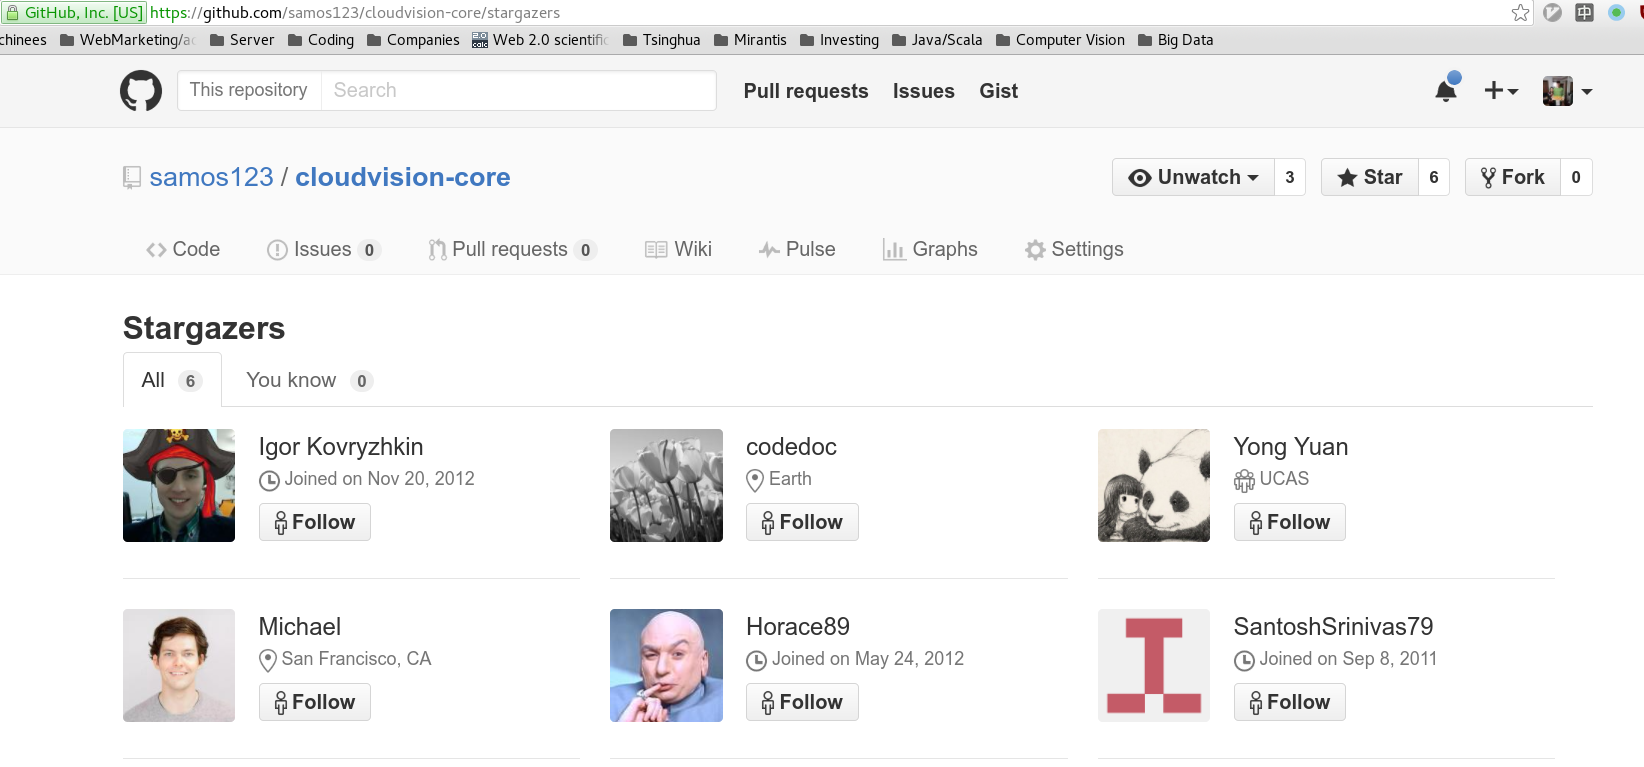
\includegraphics[width=0.49\textwidth]{cloudvision-github-stars}
    \caption{CloudVision在GitHub获得的认可}
  \label{fig:cloudvision-github-stars}
\end{wrapfigure}
我们认为CloudVision把机器视觉的PaaS平台基础搭建好了。
在GitHub的开源软件社交网站CloudVision获得了一些认可,在图\ref{fig:cloudvision-github-stars}
可以看到GitHub里有6个用户已经点赞了,包括一个Stanford大学的研究生mdangelo。
虽然基础搭建好了但是还是得提高Spark稳定性和
集成机器视觉最近主流的深度学习。
在稳定性上,发现在Spark执行一些数据量很大的任务,经常会有Out of Memory错误,
然后直接内核杀掉进程。


\section{未来工作}
大部分软件永远完成不了,CloudVision也是这样的软件,做出来了基础但是为了跟着技术和行业的发展
CloudVision也得不停的更新。我们打算以开源的模式继续开发和维护CloudVision平台,未来
打算的工作包括:
\begin{itemize}
  \item 解决Spark稳定性问题

        在实验的时候,我们发现Spark如果长期执行大量数据的任务会发生Out of Memory异常。
        我们认为这可能是一个上游的Spark Bug,调研以后发现确实有个Spark bug。\cite{spark-oom-bug}
        Spark还没发布的2.0也会集成Tungsten,Tungsten也能解决多数的Out of Memory异常。
        未来工作包括解决以及升级CloudVision用的Spark版本,同时改进机器视觉库,使用Spark新的
        DataFrame的功能避免依赖PySpark。

  \item 集成深度学习软件

        最近深度学习达到了机器视觉多种应用最好的结果,CloudVision也需要提供
        深度学习的功能,目前有几个主流的软件,Caffe,TensorFlow,SparkNet,Deeplearning4j。
        需要调研哪个软件会变成未来的趋势,支持大规模分布式训练。前期调研认为Google开发的
        TensorFlow会变成深度学习的标准。我们打算集成TensorFlow到CloudVision里面,让用户
        通过CloudVision部署和管理TensorFlow集群,同时通过CloudVision提交TensorFlow的任务。

  \item 集成AWS和其他公有云

        CloudVision的架构和实现抽象了云平台的资源,但是目前只有集成和测试基于OpenStack API的
        云平台。未来我们也可以同样集成其他云平台,比如AWS,Azure,Google Compute Engine等等。

\end{itemize}



